\section{Introduction and Motivation}

Text-to-image diffusion models often fail on compositional prompts even when the image looks plausible: they miscount objects, swap colors, or ignore spatial relations. Common fixes such as retraining, fine-tuning, or stronger classifier-free guidance either require extra training or trade alignment against image quality. Zigzag Diffusion Sampling (Z-Sampling) is interesting because it claims to improve alignment only at inference time. The method denoises a latent, partially inverts it with a different guidance scale, and then re-denoises it. Bai et al. describe this as a form of self-reflection: the model uses its own conditional vector field twice and keeps the guidance-gap signal.

My individual lane in Group 14 tests this idea on a practical but difficult setting: \texttt{Lykon/dreamshaper-xl-v2-turbo} with a GenEval-style prompt subset. This is not the paper's headline SDXL-base or SD2.1 table setting. It asks a narrower question: if the model only has four denoising steps, does Z-Sampling still help enough to justify the extra inversion calls?

\section{Method and Implementation}

Standard DDIM sampling repeatedly predicts noise and moves from $x_t$ to $x_{t-1}$ using classifier-free guidance $\gamma$. Z-Sampling modifies the early part of this loop. At each refined timestep it first denoises with guidance $\gamma_1$, then applies a DDIM inverse step with low guidance $\gamma_2$, and finally denoises again. The key hyperparameters are the total inference steps $T$, the refined window $\lambda_{step}$, the number of zigzag rounds $t_{max}$, and the guidance pair $(\gamma_1, \gamma_2)$.

For my run I used the DreamShaper-turbo settings from the paper notes: $T=4$, $\gamma_1=3.5$, $\gamma_2=0$, $\lambda_{step}=3$, and $t_{max}=1$. Standard and Z-Sampling images share the same initial latent for every prompt--seed pair, so pairwise differences come from the sampler rather than from random initialization.

The implementation lives in \texttt{src/zigzag\_project/zsampling.py}. It is a repo-local adaptation of the upstream SDXL \texttt{z\_sampling\_call} from \texttt{xie-lab-ml/zigzag-diffusion-sampling} at commit \texttt{513eb51cef223e7a562b5eb9b31d5ac5fa6b70f4}. Two implementation details mattered. First, the inverse scheduler must be cloned from the DDIM forward scheduler so denoising and inversion use compatible timesteps. Second, repeated scheduler calls require resetting the internal step index; otherwise the inversion/re-denoising loop drifts from the intended upstream behavior. These cases are covered by the project's unit tests.

\section{Experiment Setting}

I evaluated 18 GenEval prompts: the first three prompts from each of six tags (\texttt{single\_object}, \texttt{two\_object}, \texttt{counting}, \texttt{colors}, \texttt{position}, and \texttt{color\_attr}). I used seeds 42, 123, and 2026, giving 54 paired comparisons. Images were generated at $768\times768$ on an Apple M4 Max using MPS. The software stack was Python 3.10, \texttt{torch==2.12.0}, \texttt{diffusers==0.37.1}, \texttt{transformers==5.8.1}, and \texttt{hpsv2==1.2.0}. This differs from the paper's CUDA-oriented stack, so I treat absolute scores as local reproduction evidence rather than exact upstream numbers.

I used two metrics. HPSv2.1 gives a learned human-preference score for each image. More importantly, I also ran GenEval detector-style scoring on the same 54 pairs using \texttt{mmdet==2.28.2} and \texttt{mmcv-full==1.7.2} on CPU. The detector result is closer to the paper's compositional evaluation than HPSv2, although it is still a small local subset rather than the full benchmark.

\section{Results}

The detector result is the strongest evidence. Standard sampling passes 17/54 pairs (31.5\%), while Z-Sampling passes 27/54 pairs (50.0\%), a +18.5 percentage-point gain. There are 10 Z-only detector wins and 0 standard-only detector wins. By tag, Z improves \texttt{colors}, \texttt{counting}, and \texttt{two\_object} by +33.3 percentage points each, improves \texttt{position} by +11.1 points, ties \texttt{single\_object}, and neither sampler solves \texttt{color\_attr}.

\begin{table}[t]
\centering
\caption{GenEval detector pass rates on Vlad's 54 paired images.}
\label{tab:vlad-detector}
\begin{tabular}{lrrr}
\hline
Tag & Pairs & Standard & Z-Sampling \\
\hline
color\_attr & 9 & 0 & 0 \\
colors & 9 & 5 & 8 \\
counting & 9 & 2 & 5 \\
position & 9 & 0 & 1 \\
single\_object & 9 & 9 & 9 \\
two\_object & 9 & 1 & 4 \\
\hline
Overall & 54 & 17 & 27 \\
\hline
\end{tabular}
\end{table}

HPSv2.1 agrees directionally but is more optimistic. Z-Sampling wins 53/54 HPS pairwise comparisons, with mean HPS increasing from 0.217 for standard sampling to 0.253 for Z-Sampling. The mean pairwise delta is +0.0358. Every tag has a positive mean delta, including \texttt{position}, where the HPS gain is smaller but still positive.

The main cost is runtime. Standard 4-step sampling averaged 6.16 seconds per image; Z-Sampling averaged 13.80 seconds, about 2.24$\times$ slower. To check whether Z only wins because it performs more network calls, I ran a compute-matched control: 9-step standard DDIM using the same prompts, seeds, CFG scale, image size, and initial latent construction. This baseline was slower than Z-Sampling on my MPS setup (18.14 seconds/image), and it narrowed but did not erase the result. Against 9-step standard, the existing 4-step Z-Sampling images still win 42/54 HPS comparisons with mean delta +0.0245.

% Optional figure: upload these two PNGs to Overleaf under figures/vlad_geneval/ if you want this figure.
% \begin{figure}[t]
% \centering
% \begin{minipage}{0.48\linewidth}
% \centering
% 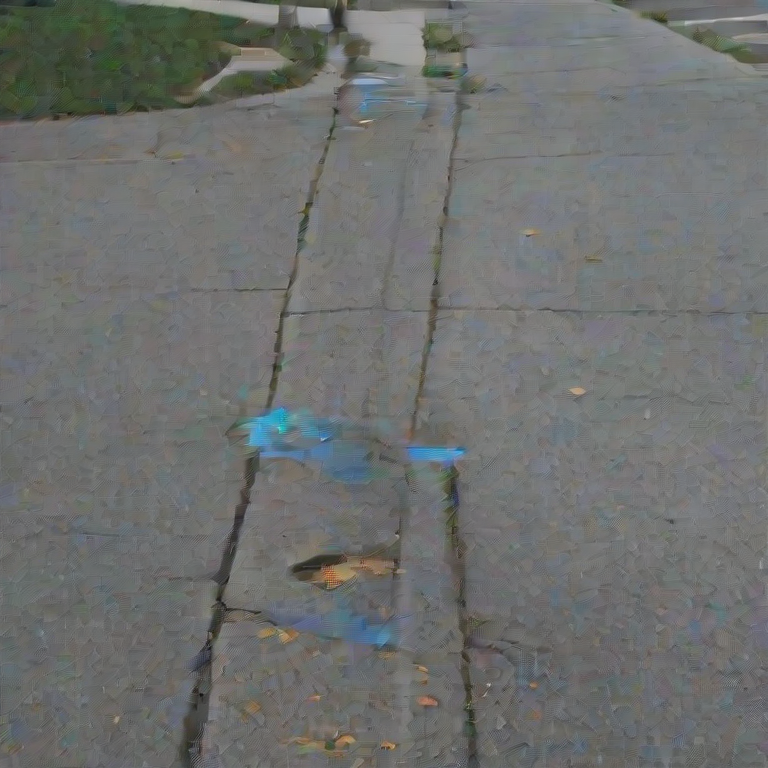
\includegraphics[width=\linewidth]{figures/vlad_geneval/geneval_259_colors_seed42_standard.png}
% Standard
% \end{minipage}\hfill
% \begin{minipage}{0.48\linewidth}
% \centering
% 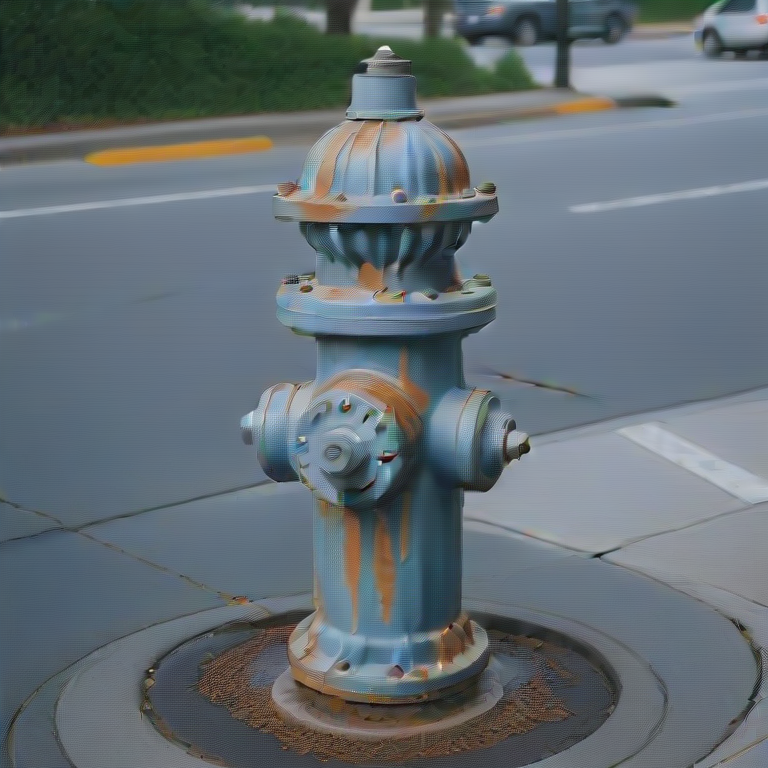
\includegraphics[width=\linewidth]{figures/vlad_geneval/geneval_259_colors_seed42_zigzag.png}
% Z-Sampling
% \end{minipage}
% \caption{Prompt ``a photo of a blue fire hydrant'' (colors, seed 42). This was the largest HPSv2 Z-Sampling win in the subset.}
% \label{fig:vlad-hydrant}
% \end{figure}

Qualitatively, the largest wins match the metrics. For example, the blue-fire-hydrant prompt becomes more clearly blue and object-focused, and the two-backpacks prompt separates the two objects more clearly. The only HPS loss is tiny (-0.0023) on a position prompt where both images are visually close.

\section{Interpretation and Limitations}

The result supports the paper's claim in my narrow lane: Z-Sampling improves a turbo DreamShaper model on a balanced GenEval subset, and the gain survives a stronger 9-step standard baseline. However, the conclusion should be reported carefully. HPSv2 can reward saturation, sharpness, and aesthetics, so the 53/54 HPS win rate is not by itself proof of better compositional reasoning. The detector result is more convincing, but it is only 54 pairs, not the full GenEval benchmark.

The tag pattern is also important. Z-Sampling helps most on color, counting, and two-object prompts. It barely helps spatial \texttt{position}, and it does not solve \texttt{color\_attr} in this subset. This suggests the method amplifies some prompt signals better than others. It is not a universal fix for every compositional failure.

Finally, the environment differs from the paper. I used modern diffusers and Apple Silicon MPS because the older CUDA stack was not practical locally. The results are therefore a reproducible local validation, with manifests, seeds, scripts, and tests committed, but not a pixel-identical reproduction of the paper environment.

\section{Conclusion}

For DreamShaper-xl-v2-turbo on my GenEval subset, Z-Sampling is useful but not free. It improves detector pass rate from 31.5\% to 50.0\%, improves HPSv2 by +0.0358 on average, and still beats a slower 9-step standard baseline on 42/54 HPS pairs. The best final claim is therefore modest: Z-Sampling gives real local gains for this turbo model, especially on colors/counting/two-object prompts, but its benefits are uneven and should be reported together with runtime cost, metric caveats, and the small-subset limitation.
